\chapter{Counterfactual Regret Minimization}
\label{chapter:cfr}

El objetivo de este capítulo es presentar un algoritmo que permita encontrar un equilibrio de Nash en juegos en forma extensiva no determinista con información incompleta y probarlo empíricamente en distintos juegos. Aunque todo juego en forma extensiva puede ser representado en forma normal, esto no es de mucho interés, pues la forma normal puede tener un tamaño exponencialmente más grande al tamaño del árbol. Se verá como el concepto de minimización del \textit{regret} puede ser extendido a juegos secuenciales, sin necesidad de la forma normal explícita. Los conceptos, procedimientos y teoremas mostrados en esta sección, son presentados en \cite{bib:cfr}.

\section{Regret Minimization}

La primera definición clave es el \textit{regret}. Para esto, es necesario considerar jugar repetidamente un juego en forma extensiva. Sea $\sigma_i^t$ la estrategia usada por el jugador $i$ a tiempo $t$. La Definición \ref{def:average-overall-regret}, presenta el concepto de \textit{regret} promedio general.

\begin{definition}
\label{def:average-overall-regret}
El \textbf{regret} promedio general del jugador $i$ a tiempo $T$ es:
\begin{alignat}{1}
R_i^T\ =\ \max_{\sigma^* \in B_i} \, \frac{1}{T}\, \sum_{t = 1}^T \, u_i(\sigma_i^*, \sigma_{-i}^t) - u_i(\sigma^t) \,.
\end{alignat}
\end{definition}

Se denotará con $\bar{\sigma}_i^{T}$ la estrategia promedio del jugador $i$ del tiempo $1$ al tiempo $T$. En particular, para cada conjunto de información $I \in \mathcal{I}_i$ y para cada acción $a \in A(I)$ se define:
\begin{alignat}{1}
\bar{\sigma}_i^{T}(I)(a)\ =\ \frac{\sum_{t = 1}^T \pi^{\sigma^t_i}(I)\sigma^t_i(I)(a)}{\sum_{t = 1}^T \pi^{\sigma_i^t}(I)} \,.
\end{alignat}

Esta estrategia es el promedio ponderado de las probabilidades $\sigma^t(I)(a)$ con respecto a que tan probable es alcanzar $I$ dado $\sigma_i^t$. La relación entre el \textit{regret} promedio general y el concepto de solución se muestra en el Teorema~\ref{theo:regret-nash}.
\begin{theorem}
\label{theo:regret-nash}
En un juego de $2$ jugadores de suma cero si el regret promedio general a tiempo $T$ es menor que $\varepsilon$ entonces $\sigma^{-T}$ es un $2\varepsilon$-equilibrio de Nash.
\end{theorem}

Como consecuencia del teorema anterior se obtiene que un algoritmo que lleve el \mbox{\textit{regret}} promedio general a cero conducirá a un equilibrio de Nash. La idea fundamental del enfoque presentado a continuación, propuesto en \cite{bib:cfr}, consiste en descomponer el \textit{regret} promedio general en un conjunto de términos aditivos de \textit{regret} que puedan ser minimizados independientemente. En particular es necesario introducir un par de conceptos nuevos, la utilidad contrafactual (Definición \ref{def:utilidad-contrafactual}) y el \textit{regret} contrafactual inmediato (Definición \ref{def:regret-inmediato}).

\begin{definition}
\label{def:utilidad-contrafactual}
La \textbf{utilidad contrafactual} es la ganancia esperada dado que el conjunto $I$ es alcanzado y todos los jugadores juegan con la estrategia $\sigma$ con excepción del jugador $i$ que juega para alcanzar $I$. Formalmente, si $\pi^{\sigma}(h, h')$ es la probabilidad de ir de la historia $h$ a la historia $h'$, entonces:
\begin{alignat}{1}
u_i(\sigma, I)\ =\ \frac{\sum_{h \in I, z \in Z} \pi^{\sigma_{-i}}(h) \pi^{\sigma}(h, z) u_i(z)}{\pi^{\sigma_{-i}}(I)} \,.
\end{alignat}
\end{definition}

Para toda acción $a \in A(I)$, se define $\sigma|_{I \rightarrow a}$ como el perfil estratégico idéntico a $\sigma$ excepto que el jugador $i$ siempre elige $a$ en el conjunto de información $I$.

\begin{definition}
\label{def:regret-inmediato}
El \textbf{regret contrafactual inmediato} es:
\begin{alignat}{1}
R_{i, \text{imm}}^T(I)\ =\  \max_{a \in A(I)} \, \frac{1}{T} \, \sum_{t = 1}^T \, \pi^{\sigma_{-i}^t}(I) \, \bigl[ u_i(\sigma^t|_{I \rightarrow a}, I) - u_i(\sigma^t, I) \bigr]\,.
\end{alignat}
\end{definition}

Intuitivamente, el \textit{regret} contrafactual inmediato es el arrepentimiento del jugador $i$ en su decisión en el conjunto de información $I$, en términos de la utilidad contrafactual, con un término de ponderación adicional para la probabilidad contrafactual que $I$ alcanzaría en esa ronda si el jugador hubiera intentado hacer eso. Usualmente, es de mayor interés el \textit{regret} cuando es positivo, por lo que se define $R_{i, \text{imm}}^{T, +} (I) = \max(R^T_{i, \text{imm}} (I), 0)$. Luego, se tiene el siguiente resultado:

\begin{theorem}
\begin{alignat}{1}
R_i^T\ \leq\ \sum_{I \in \mathcal{I}_i} R_{i, \text{imm}}^{T, +}(I) \,.
\end{alignat}
\end{theorem}

Debido a que minimizar cada \textit{regret} contrafactual inmediato minimiza el \textit{regret} promedio general, es posible enfocarse en minimizar los primeros para obtener un equilibrio de Nash.

\section{Counterfactual Regret Minimization}
\label{section:cfr}

Antes de mostrar el algoritmo principal, denominado \textit{Counterfactual Regret Minimization} (CFR) para los juegos en forma extensiva, es necesario introducir el algoritmo de \textit{Regret Matching} general. Este algoritmo puede ser descrito en un dominio donde hay un conjunto fijo de acciones $A$, una función $u^t : A \rightarrow \mathbb{R}$ y en cada ronda una distribución de probabilidad $p^t$ es elegida.

\begin{definition}
\label{def:regret}
El \textit{regret} de no haber elegido la acción $a \in A$ hasta tiempo $T$, se define como:
\begin{alignat}{1}
R_i^T(a)\ =\ \frac{1}{T} \sum_{t = 1}^T \left[u_i(a) - \sum_{a' \in A}p^t(a)u^t(a)\right] \,.
\end{alignat}
\end{definition}

Se define $R^{t, +}(a) = \max(R^t(a), 0)$. Luego la distribución $p^{t+1}$ es elegida de la siguiente manera:
\begin{alignat}{1}
p^t(a)\ =\ 
\begin{cases}
\frac{R_i^{t, +}}{\sum_{a' \in A} R^{t, +}(a)}\ & \text{si }\ \sum_{a' \in A} R^{t, +}(a) > 0 \,, \\
\frac{1}{|A|}\ & \text{en otro caso} \,.
\end{cases}
\end{alignat}

\begin{theorem}
Si $|u| = \max_{t \in \{1, 2, ... T\}} \max_{a, a' \in A}(u^t(a) - u^t(a'))$ entonces el regret del algoritmo de regret matching está acotado por:
\begin{alignat}{1}
max_{a \in A}R^t(a)\ \leq\ \frac{|u| \sqrt{|A|}}{\sqrt T} \,.
\end{alignat}
\end{theorem}

Luego, el algoritmo de \textit{Counterfactual Regret Minimization} es una aplicación del algoritmo \textit{Regret Minimization} de forma independiente a cada conjunto de información. En particular, se mantiene, para cada $I \in \mathcal{I}_i$ y para todo $a \in A(I)$:
\begin{alignat}{1}
R_i^T(I, a)\ =\ \frac{1}{T} \sum_{t = 1}^T \pi^{\sigma^t_{-i}}(I)[u_i(\sigma^t|_{I \rightarrow a}, I) - u_i(\sigma^t, I)]
\end{alignat}

Se define $R_i^{T, +}(I, a) = \max(R_i^T(I, a), 0)$, luego a tiempo $T+1$ la estrategia elegida es:
\begin{alignat}{1}
\label{eq:cfr-regret-matching}
\sigma_i^{T+1}(I)(a)\ =\
\begin{cases}
\frac{R_i^{T, +}(I, a)}{\sum_{a' \in A(I) R_i^{T, +}(I, a')}}\ & \text{si } \sum_{a' \in A(I) R_i^{T, +}(I, a')} > 0 \,, \\
\frac{1}{|A(I)|}\ & \text{en otro caso.} 
\end{cases}
\end{alignat}

Este algoritmo consiste en seleccionar las acciones de forma proporcional a la cantidad del \textit{regret} contrafactual positivo de no haber elegido esa acción. Si ninguna de estas cantidades es positiva, entonces la acción se elige con una distribución uniforme. Luego, como cota de convergencia, se tiene el siguiente teorema:
\begin{theorem}
Si el jugador $i$ selecciona las acciones de acuerdo al procedimiento anterior, entonces $R^T_{i, \text{imm}}(I) \leq \Delta_{u, i} \frac{\sqrt{|A_i|}}{\sqrt{T}}$ y por lo tanto $R_i^T \leq \Delta_{u, i} |\mathcal{I}_i| \frac{|A_i|}{\sqrt T}$, donde $|A_i| = max_{h : P(h) = 1}{|A(h)|}$.
\end{theorem}


\section{Monte Carlo Conterfactual Regret Minimization}

En la Sección \ref{section:cfr} se explicó el algoritmo de CFR, utilizado para resolver juegos en forma extensiva. Sin embargo, en la versión presentada es necesario recorrer el árbol completo en cada iteración, esta versión suele conocerse como \textit{vanilla} CFR. En \cite{bib:montecarlo-cfr} se describe una familia general de algoritmos CFR (basados en muestreo) denominada Monte Carlo Conterfactual Regret Minimization (MCCRF), para evitar recorrer el árbol completo en cada iteración.

La idea general es restringir los estados terminales alcanzados en cada iteración, pero manteniendo el mismo valor esperado para la utilidad contrafactual. Dada la definición \ref{def:informacion-incompleta}, sea $\mathcal{Q} = \{Q_1, Q_2, ..., Q_r\}$, un conjunto de subconjuntos de $Z$ tal que su unión sea igual a $Z$. Cada uno de estos conjuntos será llamado un bloque. Sea $q_j > 0$ la probabilidad de considerar el bloque $Q_j$ para la iteración actual (donde $\sum_{j = 1}^r {q_j} = 1$). 
Sea $q(z) = \sum_{j | j \in Q_i}$, es decir, $q(z)$ es la probabilidad de considerar $z$ en la iteración actual. La utilidad contrafactual muestreada, cuando se actualiza el bloque $j$ es:
\begin{alignat}{1}
\tilde{u}_i(\sigma, I | j)\ =\ \sum_{h \in I, z \in Q_j} \frac{\pi^{\sigma_{-i}}(h) \pi^{\sigma}(h, z) u_i(z)}{q(z) \pi^{\sigma_{-i}}(I)} \,.
\end{alignat}

\begin{theorem}
\label{theo:esperanza-MCCFR}
$E_{j \sim q_j} [\tilde{u}_i(\sigma, I | j)]\ =\ u_i(\sigma, I)$.
\end{theorem}

Si se elige $\mathcal{Q} = {Z}$, es decir un único bloque con todas las historias terminales y $q_1 = 1$, la utilidad contrafactual es igual a la utilidad contrafactual muestreada y se obtiene el algoritmo \textit{vanilla} CFR. Si se eligen los bloques para incluir todas las historias terminales con la misma secuencia de acciones en los nodos de azar se obtiene el \textit{chance-sampled} CFR, siendo esta última versión la utilizada para estudiar los juegos presentados en este trabajo de grado. Se implementa el algoritmo como es detallado en \cite{bib:introductionCFR} que se presenta en el Apéndice~\ref{apex:chapter:algoritmos}.

% \section{Evaluación de estrategias y explotabilidad}


\section{Detalles de implementación y ejecución}

Los algoritmos y la representación de los juegos fueron implementados en el lenguaje de programación C++ utilizando la librería estándar y una librería adicional llamada \textit{Boost} \cite{bib:boost} para obtener funciones de hash de los diferentes tipos de datos utlizados. Para la representación de los juegos se utilizó una clase abstracta llamada \functionname{Game}, que recibe como \textit{template} los tipos para el estado, las acciones, las propiedades, los conjunto de información y el hash del juego específico.

Esta clase contiene las funciones virtuales necesarias para recorrer el árbol del juego de forma \textbf{implícita}, tales como: \functionname{actions}, que retornan las acciones del juego en el estado actual, \functionname{update\_state}, que actualiza el estado del juego dada una acción a realizar, \functionname{terminal\_state} que indica si un estado es terminal o no, \functionname{utility} que retorna la utilidad en un estado terminal, entre otras. Los algoritmos CFR y GEBR utilizan esta clase abstracta en su implementación.

Para cada tipo de juego, se creó una clase derivada de la clase \functionname{Game}, donde se implementaron las funciones según las reglas de cada juego. De esta forma se puede utilizar la misma implementación de los algoritmos para todos los juegos.

Cabe destacar que todos los juegos fueron representados mediantes árboles con la raíz como único nodo de azar. Algunos juegos tienen esta representación de forma natural, por ejemplo, el Kuhn Poker, ya que las cartas se reparten al inicio y luego se juega acorde a esa distribución, sin volver a introducir ninguna jugada aleatoria. Otros juegos pueden tener nodos de azar distintos a la raíz, sin embargo siempre es posible transformarlos a un árbol que represente el mismo juego donde todos los nodos de azar son condensados en la raíz y cada hijo de la raíz representa una elección por cada uno de los nodos de azar del árbol original. En esta representación se asume que todas las decisiones aleatorias se toman al inicio del juego.

La clase \functionname{Game} y todos los algoritmos son implementados suponiendo la raíz como único nodo de azar del juego. Además, se omiten los conjuntos de información donde existe una única acción posible, ya que en estos casos no hay ninguna decisión que tomar. Las ejecuciones de los algoritmos se realizaron en \textit{Amazon Web Services} (AWS), utilizando el servicio \textit{Amazon Elastic Compute Cloud} (Amazon EC2), instanciando máquinas virtuales con las siguientes caracteríscas:
\begin{itemize}[noitemsep]
    \item Procesador: Intel Broadwell E5-2686v4 2.3 GHz.
    \item 8CPUs.
    \item 32GB de memoria RAM.
    \item Sistema Operativo: Amazon Linux 2 AMI (HVM).
\end{itemize}

Para probar los algoritmos se implementaron tres clases de juegos diferentes: \textit{One Card Poker} (OCP), \textit{Dudo}, un juego de dados, y una versión del juego de dominó para $2$ personas. Se crearon varias instancias por clase de acuerdo a los parámetros de inicialización que reciben cada uno de ellas. Para la resolución de cada instancia se utilizó el algoritmo de CFR y se iteró sobre el árbol durante $10$ horas aproximadamente. Una vez terminado el tiempo asignado se calculó la mejor respuesta para cada jugador y la explotabilidad. Una instancia de un juego se considerará resuelta si la explotabilidad de la estrategia obtenida es menor que el $1\%$ de la mínima unidad de utilidad posible según cada juego.

Para evaluar la convergencia de los algoritmos y la estrategia obtenida se utilizaron las métricas de \textit{regret} y explotabilidad, respectivamente. Para calcular la explotabilidad en estos juegos se implementó el algoritmo propuesto en \cite{bib:thesis-marc-lanctot}, denominado \textit{Generalized Expectimax Best Response} (GEBR), descrito en el Apéndice~\ref{apex:chapter:algoritmos}. La complejidad de este algoritmo es $\mathcal{O}(ND)$ donde $N$ es el número de nodos del árbol y $D$ es la profundidad del árbol. Note que el algoritmo tiene una alta complejidad, por lo que se usará únicamente para calcular la explotabilidad de la estrategia final.

Por cada juego se presenta una tabla que resume los resultados, estas tablas contienen el número de nodos del árbol ($N$), el número de conjuntos de información ($I$), el valor del juego usando la estrategia obtenida ($u({\sigma})$) y la explotabilidad ($\varepsilon_{\sigma}$). Se agrega además, en cada tabla, el número de iteraciones realizadas durante el tiempo de entrenamiento y la última columna indica si el juego fue resuelto o no, según lo establecido en el párrafo anterior. Por último, también se muestra la gráfica del \textit{regret} con respecto al número de iteraciones de alguna de las instancias de cada juego. Las gráficas completas pueden ser encontradas en el Apéndice~\ref{apex:chapter:experimentos-cfr}.

\subsection*{Juego de One-Card Poker}
\textit{One-Card Poke}r, abreviado OCP(N), es la versión generalizada del juego Kuhn Póker, explicado en el Capítulo \ref{section:kuhn-poker}. En este juego, cada jugador recibe una carta de un mazo de $N$ cartas y luego pueden apostar o retirarse según las mismas reglas del Kuhn Poker. Note que OCP(3) es equivalente al Kuhn Poker. El árbol de este juego tiene $9N(N-1)+1$ nodos (incluyendo el nodo inicial, que es el nodo de azar) y hay $4N$ conjuntos de información entre ambos jugadores. 

La Tabla \ref{table:resultados-CFR-OCP} muestra un resumen de los resultados de las instancias del juego OCP. Se observa que se lograron resolver todas los casos propuestos. La Gráfica~\ref{fig:cfr-regret-ocp-200} muestra el \textit{regret} con respecto al número de iteraciones en el juego OCP$(200)$. Se observa que al principio el regret aumenta, esto debido a que el regret se inicializa en $0$ y empieza a aumentar a medida que se descubren los conjuntos de información. Luego, se observa como converge a $0$ a medida que transcurren las iteraciones.

\begin{table}[h]
    \centering
    \caption{Resultados del algoritmo CFR en el juego OCP.}
    \label{table:resultados-CFR-OCP}
    \begin{tabular}{lrrrrrc}
        \toprule
        Juego & $N$ & $I$ & Iteraciones & $u(\sigma)$ & $\varepsilon_{\sigma}$ (\%) & Resuelto \\ \midrule
        OCP$(3)$        &          55 &      12 & 1.181.763.638 & -0.056 & 0.0098 & \cmark \\
        OCP$(12)$       &       1.189 &      48 & 1.147.919.240 & -0.062 & 0.0032 & \cmark \\
        OCP$(50)$       &      22.051 &     200 & 1.145.291.974 & -0.058 & 0.0099 & \cmark \\
        OCP$(200)$      &     358.201 &     800 & 1.128.993.847 & -0.056 & 0.0078 & \cmark \\
        OCP$(1000)$     &   8.991.001 &   4.000 & 1.087.573.694 & -0.056 & 0.0098 & \cmark \\
        OCP$(5000)$     & 224.955.001 &  20.000 & 1.038.367.354 & -0.056 & 0.0241 & \cmark \\
        \bottomrule
    \end{tabular}
\end{table}

\begin{figure}[h]
    \centering
    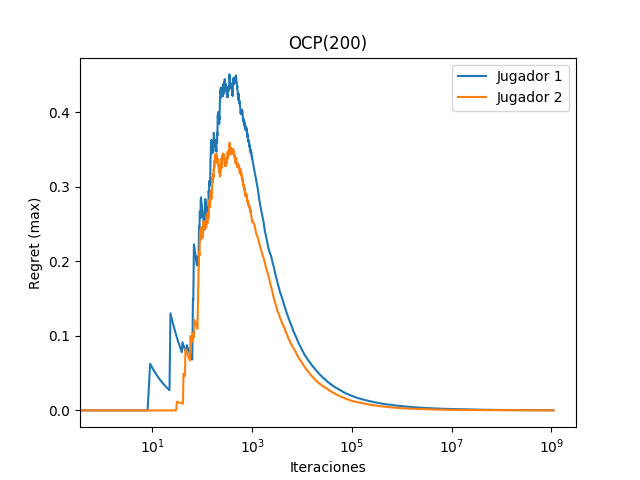
\includegraphics[width=0.5\textwidth]{graficas/cfr/ocp/OCP(200).png}
    \caption{Gráficas del \textit{regret} con respecto al número de iteraciones del juego \textit{One Card Poker} $(200)$.}
    \label{fig:cfr-regret-ocp-200}
\end{figure}

\subsection*{Juego de Dudo}
Dudo, también conocido como \textit{Bluff}, \textit{Liar's Dice} o Perudo, es un juego de dados y apuestas. Usualmente se juega entre $2$ y $6$ jugadores. Los jugadores se ubican en forma circular y cada uno de ellos tiene un número de dados. De forma simultánea, todos lanzan sus dados, cada jugador puede ver el resultado de sus propios dados, pero no puede ver el resultado de los dados de los otros jugadores. Una vez hecho esto, los jugadores empiezan a apostar sobre el número de veces que apareció una cara en específico en todos los dados que hay en la mesa.

Una apuesta consiste en decir $2$ números $(x, y)$, esto indica que el jugador apuesta que hay, al menos, $x$ dados cuyo resultado fue el número $y$. El primer jugador (que se elige previamente mediante el lanzamiento de $1$ dado o de alguna otra forma), realiza la primera apuesta y, en sentido horario, cada jugador puede hacer una apuesta más alta o decir \say{dudo} y retar al jugador anterior. Una apuesta es más alta que otra si el número de dados que se anuncian en la apuesta ($x$) es mayor, o si el número de dados es igual, pero la cara apostada ($y$) es mayor. Por ejemplo $(3, 1)$ es mayor que $(2, 5)$, y ambas apuestas son mayores que $(2, 3)$.

Por otra parte, si un jugador reta al jugador previo, se descubren todos los dados de todos los jugadores. Si la cantidad de dados con la cara $y$ es mayor o igual a $x$, donde $(x, y)$ fue la apuesta realizada por el jugador, el jugador que hizo el reto pierde un dado. En caso contrario, el jugador que hizo la apuesta pierde un dado. Luego, todos los jugadores lanzan sus dados nuevamente y una nueva ronda de apuestas empieza por el jugador que perdió la ronda anterior. Un jugador pierde cuando se queda sin dados, el ganador es el último jugador con al menos un dado restante. La figura \ref{fig:dudo} muestra una foto del juego, de \textit{Perudo}, una versión comercial de este juego, que está diseñada para $6$ jugadores, donde cada jugador empieza con $5$ dados. En la figura se observan los vasos que se utilizan para lanzar los dados y evitar que cada jugador vea los dados de los demás.

\begin{figure}[h]
    \centering
    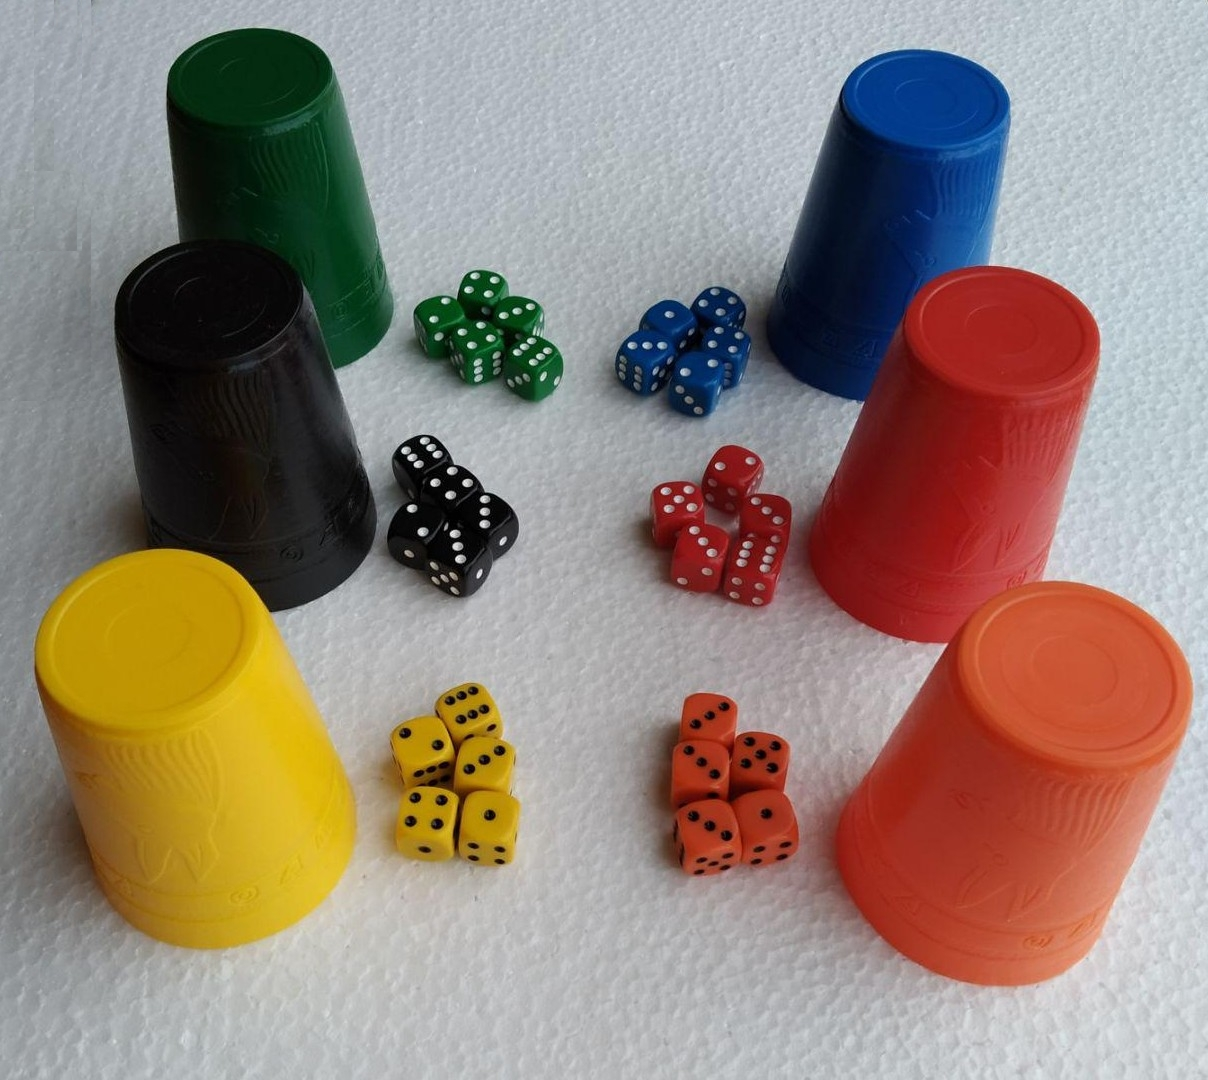
\includegraphics[width=0.4\textwidth]{figuras/dudo.jpg}
    \caption{Juego dudo. Los vasos se utilizan para lanzar los dados y evitar que los oponentes vean el resultado.}
    \label{fig:dudo}
\end{figure}

En este trabajo de grado consideraremos este juego para $2$ jugadores únicamente. Dudo$(K, D_1, D_2)$ hará referencia a una única ronda de apuestas de $2$ jugadores, donde el primer jugador tiene $D_1$ dados, el segundo jugador tiene $D_2$ dados y cada dado tiene $K$ caras. El juego completo consiste en múltiples rondas, donde $D_1$ o $D_2$ disminuye en una unidad al finalizar cada ronda. Cuando uno de los jugadores pierde todos los dados obtiene una utilidad de $-1$, mientras que su oponente obtiene una utilidad de $1$. En este juego cada ronda se considerará un subjuego y se representará con un árbol independiente, donde los valores esperados para los juegos Dudo$(K, D_1 - 1, D_2)$ y Dudo$(K, D_1, D_2 - 1)$ se precalculan y se utilizan como utilidad para las hojas del árbol Dudo$(K, D_1, D_2)$. Note que, en el juego estándar, $K$ siempre tiene un valor de $6$.

Cuando el jugador $i$ lanza $D_i$ dados hay $\binom{D_i+K-1}{K-1}$ resultados diferentes posibles, ya que cada resultado puede ser representado con una tupla $(a_1, a_2, ..., a_k)$, donde $a_j$ representa el número de dados con la cara $j$, por lo que $\sum_j^K = D_i$ y $a_j \geq 0$. Por otra parte cada secuencia de apuestas puede ser representada por una secuencia binaria de longitud $K(D_1 + D_2)$, donde el $i$-ésimo bit es $1$ si la $i$-ésima secuencia más alta fue dicha durante la ronda y $0$ en caso contrario. Por ejemplo, si $D_1 = D_2 = 1$, las apuestas $(1, 1)-(1, 3)-(1, 6)-(2, 4)-(2, 5)-(1, 6)$ se representa con la secuencia binaria $101001000110$, por lo que hay $2^{K(D_1 + D_2)}$ secuencias diferentes. Cada secuencia pertenece a un jugador en específico, por lo que si $D_1 = D_2$, el número de conjuntos de información  es igual a  $\binom{D_i+K-1}{K-1}2^{K(D_1 + D_2)}$, incluyendo los conjuntos de información con una única acción posible. Para excluir estos conjuntos de información, debemos excluir las secuencias donde la última apuesta es la máxima apuesta posible, pues el siguiente jugador sólo podría decir \say{dudo}. La cantidad de estas secuencias es igual a $2^{K(D_1 + D_2)-1}$, luego, el número de conjuntos de información con más de una acción posible es igual a $\binom{D_i+K-1}{K-1}2^{K(D_1 + D_2)-1}$, dado que ambos jugadores tienen el mismo número de dados.

Para contar el número total de nodos, se puede considerar el lanzamiento de los dados de forma independiente, pues las secuencias posibles de apuestas no dependen del resultado de los dados. Por lo expuesto anteriormente el número posible de apuestas es igual a $2^{K(D_1+D_2)}$, pero después de cada secuencia siempre se puede decir \say{dudo}, salvo para la secuencia vacía. Luego el número total de nodos (incluyendo nodos terminales y no terminales) es igual a $\binom{D_1+K-1}{K-1}\binom{D_1+K-1}{K-1}(2^{K(D_1+D_2)+1}-1)+1$.

La Tabla~\ref{table:resultados-CFR-dudo} muestra el resumen de los resultados de las instancias del juego dudo. En este juego no se alcanzó la cota deseada para la explotabilidad para las instancias Dudo$(4, 2, 2)$, Dudo$(5, 2, 2)$, Dudo$(6, 1, 2)$ y Dudo$(6, 2, 1)$, siendo la instancia Dudo$(5, 2, 2)$ la que posee la estrategia más explotable con más del $15\%$ de la ganancia posible, esto debido al bajo número de iteraciones realizadas durante el entrenamiento (menos de $4000$), debido al gran tamaño del árbol. La Gráfica~\ref{fig:cfr-regret-dudo-5-2-2} corresponde al juego Domino$(5, 2, 2)$, ésta tiene un comportamiento similar a la gráfica anterior, sin embargo, se observa que la convergencia está inconclusa, por lo que la estrategia tiene alta explotabilidad.

\begin{table}[h]
    \centering
    \caption{Resultados del algoritmo CFR en el juego dudo.}
    \label{table:resultados-CFR-dudo}
    \begin{tabular}{lrrrrrc}
        \toprule
        Juego & $N$ & $I$ & Iteraciones & $u(\sigma)$ & $\varepsilon_{\sigma}$ (\%) & Resuelto \\ \midrule
        Dudo$(3, 1, 1)$ &         1.144 &          96 & 77.243.464 & -0.111 &  0.0098 & \cmark \\
        Dudo$(3, 1, 2)$ &        18.415 &       1.152 & 10.050.143 & -0.465 &  0.0211 & \cmark \\
        Dudo$(3, 2, 1)$ &        18.415 &       1.152 &  9.903.467 &  0.506 &  0.0111 & \cmark \\
        Dudo$(3, 2, 2)$ &       294.877 &      12.288 &  1.137.993 & 0.0054 &  0.2887 & \cmark \\
        Dudo$(4, 1, 1)$ &         8.177 &         512 & 18.697.532 & -0.125 &  0.0259 & \cmark \\
        Dudo$(4, 1, 2)$ &       327.641 &      14.366 &  1.215.600 & -0.508 &  0.0971 & \cmark \\
        Dudo$(4, 2, 1)$ &       327.641 &      14.366 &  1.213.799 &  0.552 &  0.3701 & \cmark \\
        Dudo$(4, 2, 2)$ &    13.107.101 &     327.680 &     63.109 & 0.0069 &  2.1132 & \xmark \\
        Dudo$(5, 1, 1)$ &        51.176 &       2.560 &  4.521.208 & -0.120 &  0.1186 & \cmark \\
        Dudo$(5, 1, 2)$ &     4.915.126 &     163.840 &    151.235 & -0.565 &  0.6197 & \cmark \\
        Dudo$(5, 2, 1)$ &     4.915.126 &     163.840 &    143.698 &  0.581 &  0.0122 & \cmark \\
        Dudo$(5, 2, 2)$ &   471.858.976 &   7.864.320 &      3.826 &  0.836 & 15.1963 & \xmark \\
        Dudo$(6, 1, 1)$ &       294.877 &      12.288 &  1.067.782 & -0.111 &  0.0975 & \cmark \\
        Dudo$(6, 1, 2)$ &    66.060.163 &   1.769.472 &     17.702 & -0.593 &  4.5781 & \xmark \\
        Dudo$(6, 2, 1)$ &    66.060.163 &   1.769.472 &     17.221 &  0.592 &  3.9594 & \xmark \\
        \bottomrule
    \end{tabular}
\end{table}

\begin{figure}[h]
    \centering
    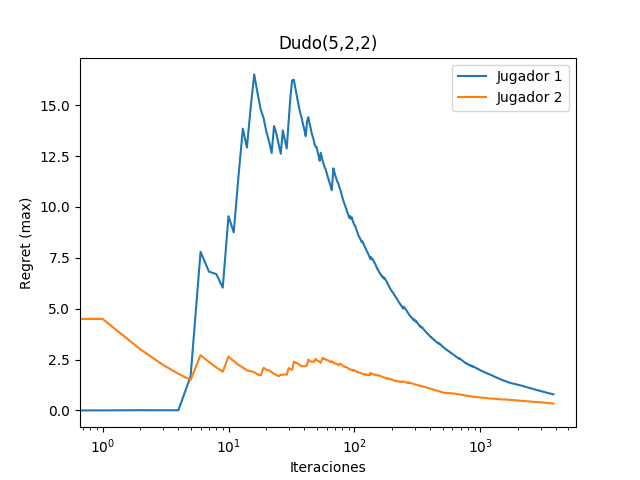
\includegraphics[width=0.5\textwidth]{graficas/cfr/dudo/Dudo(5,2,2).png}
    \caption{Gráficas del \textit{regret} con respecto al número de iteraciones del juego Dudo $(5, 2, 2)$.}
    \label{fig:cfr-regret-dudo-5-2-2}
\end{figure}

\subsection*{Juego de Dominó}
En este trabajo se utilizó una versión de este juego para $2$ jugadores. Al inicio del juego cada jugador toma una cantidad específica de piezas de forma aleatoria, las piezas restantes se dejan sin descubrir para ser usadas en turnos posteriores. Al igual que en el juego tradicional de dominó, los jugadores juegan por turnos alternados (el primero jugador se elige de forma arbitraria), cada uno debe colocar una ficha válida acorde a las reglas \textit{estándares} en Venezuela del juego. Si un jugador no puede colocar una ficha toma una ficha de las que no están descubiertas (si todavía hay disponibles), el jugador verifica si puede colocar la ficha tomada y en caso contrario pasa el turno y juega el oponente.

El juego termina cuando alguno de los jugadores usa todas las piezas o cuando ambos jugadores no pueden jugar ni tomar piezas nuevas, en este último caso se dice que el juego está bloqueado. El ganador es el jugador que se queda sin piezas o, en caso de bloqueo, el jugador que acumule menos puntos en todas las piezas que quedaron en su mano. La utilidad obtenida es el número de puntos que el jugador perdedor acumuló en las piezas que quedaron en su mano (con signo positivo para el jugador ganador y signo negativo para el perdedor). Cabe destacar que sólo se puede tomar una pieza o pasar, si no se puede realizar una jugada con la mano actual.

Usualmente se utilizan $28$ piezas, donde las piezas pueden tener entre $0$ y $6$ puntos en cada extremo, y cada jugador recibe $7$ piezas al inicio del juego. En este trabajo se parametriza el número máximo de puntos que puede tener una ficha, así como la cantidad de piezas repartidas inicialmente. De esta forma se hará referencia a Domino$(M, N)$ a un juego donde las piezas tienen entre $0$ y $M$ puntos (con un total de $(M+1)(M+2)/2$ piezas) y cada jugador recibe $N$ piezas al inicio del juego.

En este juego no es fácil calcular el tamaño del árbol y el número de conjuntos de información, principalmente porque las acciones posibles en un estado dependen tanto de la mano del jugador, como de las piezas en la mesa. En el Kuhn Poker siempre hay $2$ acciones posibles (${pasar, apostar}$) y en el Dudo las acciones disponibles dependen únicamente de la última apuesta y no dependen de los dados que tengan los jugadores. Así que estos parámetros fueron determinados recorriendo el árbol del juego mediante DFS.

La Tabla~\ref{table:resultados-CFR-domino} muestra el resumen de los resultados del juego dominó. En este caso no fue posible resolver la instancia Domino$(3, 4, 4)$ con respecto a los juegos de dominó. La Gráfica~\ref{fig:cfr-regret-domino-3-3} muestra el \textit{regret} con respecto al número de iteraciones del juego Domino$(3, 3)$, al igual que en las gráficas anteriores, se observa como el regret crece al principio para luego converger a $0$.

\begin{table}[h]
    \centering
    \caption{Resultados del algoritmo CFR en el juego dominó.}
    \label{table:resultados-CFR-domino}
    \begin{tabular}{lrrrrrc}
        \toprule
        Juego & $N$ & $I$ & Iteraciones & $u(\sigma)$ & $\varepsilon_{\sigma}$ (\%) & Resuelto \\ \midrule
        Domino$(2, 2)$ &         7.321 &     102 & 585.191.577 & 2.4    & 0      & \cmark \\
        Domino$(3, 2)$ &    46.534.657 &  88.947 & 436.905.363 & 2.8767 & 0.0292 & \cmark \\
        Domino$(3, 3)$ &   246.760.993 & 107.854 &  79.751.183 & 2.1539 & 0.3599 & \cmark \\
        Domino$(3, 4)$ & 1.547.645.185 & 104.050 &  11.984.261 & 3.2034 & 1.3630 & \xmark \\
        \bottomrule
    \end{tabular}
\end{table}

\begin{figure}[h]
    \centering
    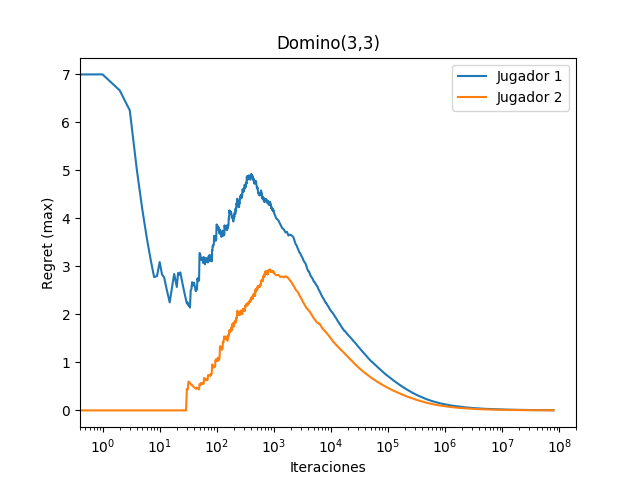
\includegraphics[width=0.5\textwidth]{graficas/cfr/domino/Domino(3,3).png}
    \caption{Gráficas del \textit{regret} con respecto al número de iteraciones del juego Dominó $(3, 3)$.}
    \label{fig:cfr-regret-domino-3-3}
\end{figure}
